

\documentclass[final,6p,times,twocolumn]{elsarticle}
\makeatletter

\renewenvironment{abstract}{\global\setbox\absbox=\vbox\bgroup
  \hsize=\textwidth\def\baselinestretch{1}%
  \noindent\unskip\textbf{Resumen}  % <--- Edit as necessary
 \par\medskip\noindent\unskip\ignorespaces}
 {\egroup}

\def\keyword{%
  \def\sep{\unskip, }%
 \def\MSC{\@ifnextchar[{\@MSC}{\@MSC[2000]}}
  \def\@MSC[##1]{\par\leavevmode\hbox {\it ##1~MSC:\space}}%
  \def\PACS{\par\leavevmode\hbox {\it PACS:\space}}%
  \def\JEL{\par\leavevmode\hbox {\it JEL:\space}}%
  \global\setbox\keybox=\vbox\bgroup\hsize=\textwidth
  \normalsize\normalfont\def\baselinestretch{1}
  \parskip\z@
  \noindent\textit{Palabras clave: }  % <--- Edit as necessary
  \raggedright                         % Keywords are not justified.
  \ignorespaces}



\usepackage[spanish]{babel}

\def\ps@pprintTitle{%
     \let\@oddhead\@empty
     \let\@evenhead\@empty
     \def\@oddfoot{\footnotesize\itshape
        \ifx\@journal\@empty   % <--- Edit as necessary
       \else\@journal\fi\hfill\today}%
     \let\@evenfoot\@oddfoot}

%% The graphicx package provides the includegraphics command.
\usepackage{graphicx}
%% The amssymb package provides various useful mathematical symbols
\usepackage{amssymb}
%% The amsthm package provides extended theorem environments
%% \usepackage{amsthm}

%% The lineno packages adds line numbers. Start line numbering with
%% \begin{linenumbers}, end it with \end{linenumbers}. Or switch it on
%% for the whole article with \linenumbers after \end{frontmatter}.
\usepackage{lineno}


%% natbib.sty is loaded by default. However, natbib options can be
%% provided with \biboptions{...} command. Following options are
%% valid:

%%   round  -  round parentheses are used (default)
%%   square -  square brackets are used   [option]
%%   curly  -  curly braces are used      {option}
%%   angle  -  angle brackets are used    <option>
%%   semicolon  -  multiple citations separated by semi-colon
%%   colon  - same as semicolon, an earlier confusion
%%   comma  -  separated by comma
%%   numbers-  selects numerical citations
%%   super  -  numerical citations as superscripts
%%   sort   -  sorts multiple citations according to order in ref. list
%%   sort&compress   -  like sort, but also compresses numerical citations
%%   compress - compresses without sorting
%%
%% \biboptions{comma,round}

% \biboptions{}

%\journal{Journal Name}

\begin{document}

\begin{frontmatter}

%% Title, authors and addresses

\title{Sistema multiagente: simulación de una epidemia}

%% use the tnoteref command within \title for footnotes;
%% use the tnotetext command for the associated footnote;
%% use the fnref command within \author or \address for footnotes;
%% use the fntext command for the associated footnote;
%% use the corref command within \author for corresponding author footnotes;
%% use the cortext command for the associated footnote;
%% use the ead command for the email address,
%% and the form \ead[url] for the home page:
%%
%% \title{Title\tnoteref{label1}}
%% \tnotetext[label1]{}
%% \author{Name\corref{cor1}\fnref{label2}}
%% \ead{email address}
%% \ead[url]{home page}
%% \fntext[label2]{}
%% \cortext[cor1]{}
%% \address{Address\fnref{label3}}
%% \fntext[label3]{}


%% use optional labels to link authors explicitly to addresses:
%% \author[label1,label2]{<author name>}
%% \address[label1]{<address>}
%% \address[label2]{<address>}

\author{Fabiola Vázquez}

\address{Facultad de Ingeniería Mecánica y Eléctrica, UANL.}

\begin{abstract}
%% Text of abstract
Durante la historia de la humanidad, esta se ha enfrentado a diversas enfermedades que terminan con la vida de gran parte de la población. Debido a esto, durante ya muchos años se han desarrollado innumerables modelos matemáticos para tratar de afrontar estos problemas. Uno de los enfoques más recientes es el uso de los llamados sistemas multiagentes, que permiten simular diferentes escenarios de propagación de enfermedades y medir los resultados de acciones para mitigar los contagios. En este trabajo se pretende mostrar el cambio que podría existir si la población hace uso del cubrebocas para evitar propagar más una enfermedad.
\end{abstract}

\begin{keyword}
Sistema multiagente \sep epidemia  \sep simulación \sep SIR 
%% keywords here, in the form: keyword \sep keyword

%% MSC codes here, in the form: \MSC code \sep code
%% or \MSC[2008] code \sep code (2000 is the default)

\end{keyword}

\end{frontmatter}

%%
%% Start line numbering here if you want
%%
%\linenumbers

%% main text
\section{Introducción}
Actualmente, a nivel global se vive con la pandemia ocasionada por el virus SARS-CoV-2 y algunas de las medidas para evitar su propagación son el uso correcto del cubrebocas, lavado de manos frecuentes y aislamiento social, es decir, no salir a menos que sea totalmente necesario. Muchas personas han hecho poco caso a las indicaciones y continuamente salen sin protección alguna ya que se cree que el uso de las medidas antes mencionadas no ayudan a reducir los contagios. El objetivo de esta experimentación es mostrar los cambios que se pueden logran obtener si se hace uso correcto del cubrebocas como medida para evitar contagios.

En la sección \ref{S:2} se explican algunos conceptos básicos, como agente, epidemia, sistema multiagente y el modelo SIR. La sección \ref{S:trela} se detalla un poco sobre los trabajos que se han realizado anteriormente sobre los sistemas multiagentes, no solo en el área de epidemiología. La sección \ref{S:Sprop} trata de como se intenta dar solución al problema mencionado anteriormente y cuales herramientas fueron utilizadas para ello. 

\label{S:1}


%\begin{itemize}
%\item Bullet point one
%\item Bullet point two
%\end{itemize}
%
%\begin{enumerate}
%\item Numbered list item one
%\item Numbered list item two
%\end{enumerate}





%\begin{table}[h]
%\centering
%\begin{tabular}{l l l}
%\hline
%\textbf{Treatments} & \textbf{Response 1} & \textbf{Response 2}\\
%\hline
%Treatment 1 & 0.0003262 & 0.562 \\
%Treatment 2 & 0.0015681 & 0.910 \\
%Treatment 3 & 0.0009271 & 0.296 \\
%\hline
%\end{tabular}
%\caption{Table caption}
%\end{table}




%\begin{figure}[h]
%\centering\includegraphics[width=0.4\linewidth]{placeholder}
%\caption{Figure caption}
%\end{figure}





\section{Antecedentes}
Existen diversas maneras de definir un agente. Según la Real Academia Española, un agente es una persona o cosa que produce un efecto. Una de las características principales que posee un agente es su autonomía, es decir, que poseen la capacidad de tomar decisiones independientemente sin intervención alguna de uno o más agentes. Además poseen capacidad de inferencia, es decir que son capaces de observar de forma general la información. En los sistemas que se muestran, cada uno de los agentes \cite{introductionmas} posee sus propias características, como lo puede ser la posición inicial, su estado actual, si posee enfermedades previas, etcétera.   

Un sistema multiagente \cite{surveymas} es un sistema donde un grupo de agentes autónomos interactúan en un entorno. Este tipo de sistemas han sido adaptados en diversas áreas debido a que, cuando se utiliza cómputo paralelo, este tipo de sistemas incrementa la velocidad y la eficiencia de la simulación.

Un modelo epidemiológico de tipo SIR es un modelo con compartimentos donde cada agente puede estar en uno de tres estados: susceptible, infectado o recuperado. El agente solo puede pasar de susceptible a infectado (al ser contagiado), o de infectado a recuperado, donde se asume desarrolla inmunidad a la infección. La figura \ref{sir} muestra los cambios del estado del agente.
\begin{figure}
\label{sir}
\centering
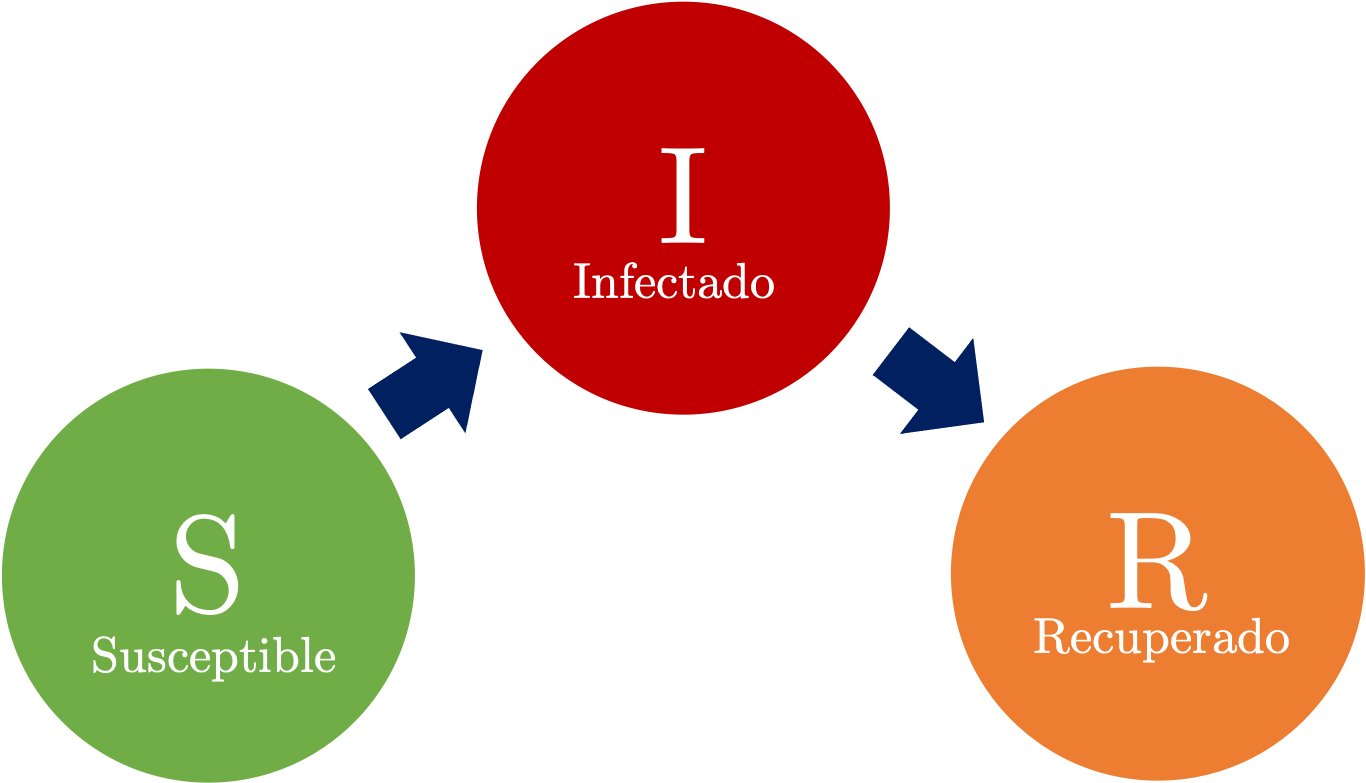
\includegraphics[scale=0.2]{sir.png}
\caption{Modelo SIR.}
\end{figure}





\label{S:2}



%% The Appendices part is started with the command \appendix;
%% appendix sections are then done as normal sections
%% \appendix

%% \section{}
%% \label{}

%% References
%%
%% Following citation commands can be used in the body text:
%% Usage of \cite is as follows:
%%   \cite{key}          ==>>  [#]
%%   \cite[chap. 2]{key} ==>>  [#, chap. 2]
%%   \citet{key}         ==>>  Author [#]

\section{Trabajos relacionados}
\label{S:trela}
Las investigaciones que involucran el uso de agentes comenzaron a principios de los años ochenta. En el año de 1990, Varian \cite{Varian} investigó un problema del ámbito económico donde los agentes pueden monitorear el comportamiento de otros agentes. 
En teoría de juegos el uso de sistemas multiagentes es muy usado, por ejemplo, Pendharkar  \cite{gametheoretical} estudió el comportamiento cooperativo y competitivo de los agentes y trabajó también con conceptos del área de economía. En el área de epidemiología se tienen trabajos como el de Swarup \cite{Swarup} el cual describe el estado del arte de los sistemas multiagente en esta área en particular y muestra algunos problemas que aún no han sido resueltos. 
\section{Solución propuesta}
\label{S:Sprop}
Se trabaja con el software libre R \cite{R} en un cuaderno de Jupyter \cite{jupyter}. El entorno de los agentes se considera como el cuadrado de lado 1.5 $\times$ 1.5 donde estos se posicionan uniformemente pseudo al azar. Se considera también dos experimentos diferentes, en cada uno se trabajan con 50 agentes y un tiempo de 100. En la figura \ref{paso1} se muestra el estado inicial de los agentes en el entorno, donde los agentes de color rojo son los infectados, los verdes son los susceptibles y los triángulos invertidos son los agentes que están vacunados. 

\begin{figure}
\label{paso1}
\centering
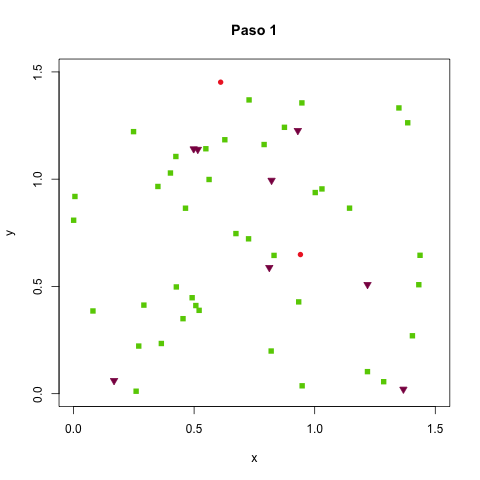
\includegraphics[scale=0.4]{p6_t001.png}
\caption{Estado inicial de los agentes en su entorno.}
\end{figure}

En el primer experimento, los agentes pueden ser vacunados con una probabilidad \texttt{pv} y estos adquieren el estado de recuperado y no puede ser infectado nuevamente. En el segundo experimento, los agentes también pueden ser vacunados, pero se considera la probabilidad de 0.05 de que la vacuna falle, es decir, si el agente está vacunado y éste entra en contacto con alguien infectado, existe la posibilidad de volverse a contagiar; además se incluye que los agentes usan o no un cubrebocas para disminuir los contagios, esto se decide pseudo al azar. 
\begin{figure}
\label{sinmasc}
\centering
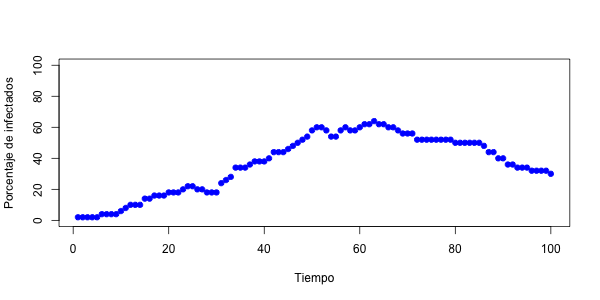
\includegraphics[scale=0.4]{sinmasc.png}
\caption{Ejemplo de una corrida considerando que los agentes se pueden vacunar, en este caso no se contempla el uso de cubrebocas.}
\end{figure}
\begin{figure}
\label{conmasc}
\centering
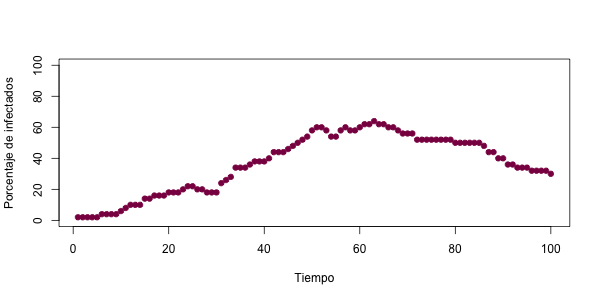
\includegraphics[scale=0.4]{conmasc.png}
\caption{Ejemplo de una corrida considerando que los agentes vacunados pueden ser nuevamente susceptibles, en este caso se contempla el uso de cubrebocas.}
\end{figure}
La figura \ref{sinmasc} muestra el comportamiento de la epidemia en una sola corrida para el experimento 1 y la figura \ref{conmasc} muestra dicho comportamiento pero referente al experimento 2. Con una sola corrida no se puede ver el cambio que hay si el agente usa cubrebocas o no. 


Se realiza la simulación variando la probabilidad \texttt{pv} de que un agente se pueda vacunar para ver el comportamiento en los dos experimentos mencionados anteriormente. La figura \ref{sinmasc1} muestra los gráficos de caja obtenidos con el experimento 1 y la figura \ref{conmasc1} los del experimento 2. Como se puede apreciar en dichas figuras, el comportamiento es similar, mientras mayor sea la probabilidad de que el agente se vacune, menor será el porcentaje de infectados. La figura \ref{conmasc1} comienza con un porcentaje mayor de infectados comparado con la figura \ref{sinmasc1} y esto es debido que en el segundo experimento, aún vacunado el agente, existe la probabilidad de que esta falle y sea contagiado. 

\begin{figure}
\label{sinmasc1}
\centering
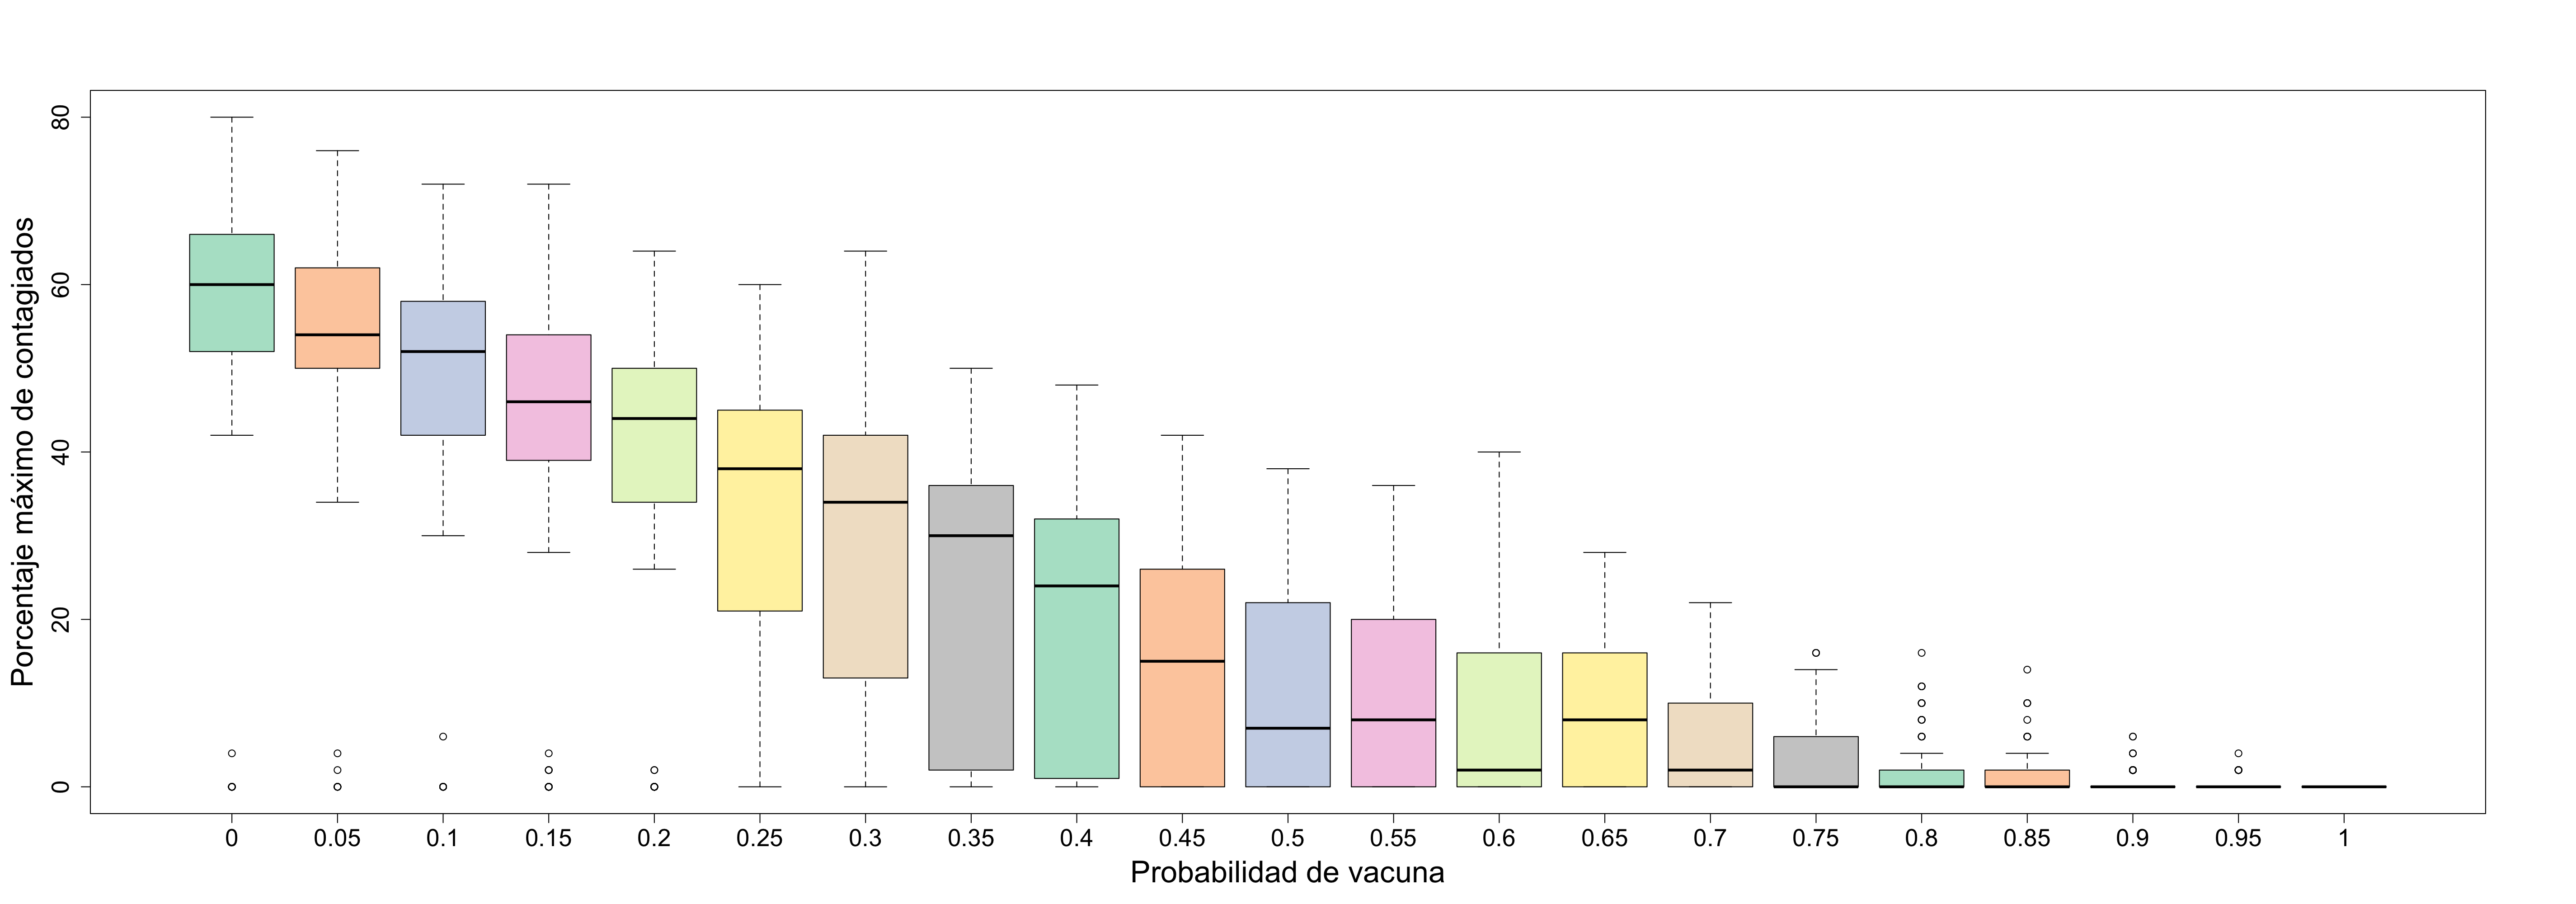
\includegraphics[width=\linewidth]{boxplot1.png}
\caption{Gráficos de caja variando la probabilidad de que un agente se vacune en el experimento 1.}
\end{figure}

\begin{figure}
\label{conmasc1}
\centering
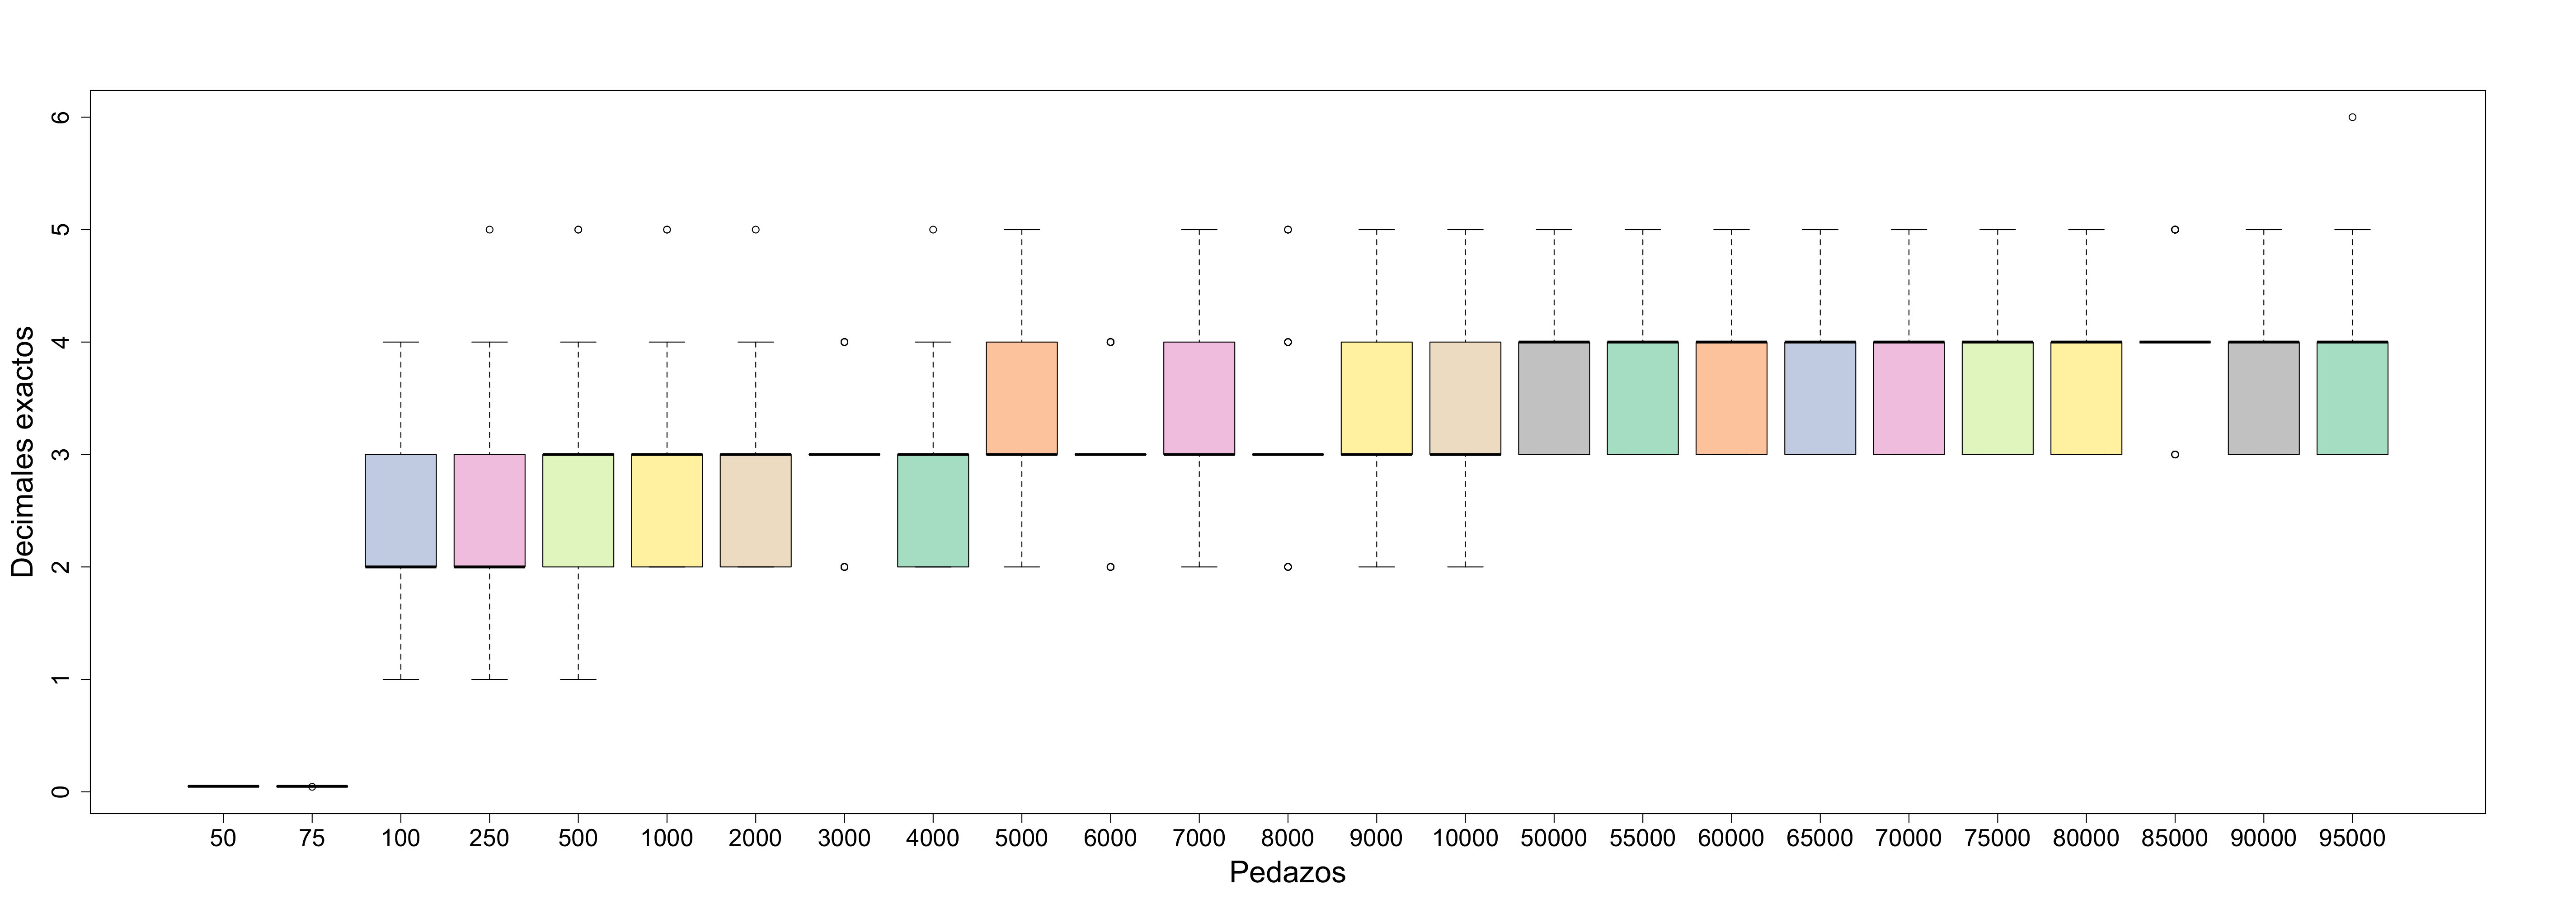
\includegraphics[width=\linewidth]{boxplot2.png}
\caption{Gráficos de caja variando la probabilidad de que un agente se vacune en el experimento 2.}
\end{figure}

Se realiza un tercer estudio, considerando las condiciones del experimento 2 para determinar si hay un efecto si los agentes usan un cubrebocas o no. La probabilidad de que estos no lo posean se varía de 0 a 1 en saltos de 0.25. La figura \ref{conmasc2} muestra los gráficos de caja obtenidos en dicha simulación, donde se observa que si nadie usa cubrebocas los contagios aumentan.
\begin{figure}
\label{conmasc2}
\centering
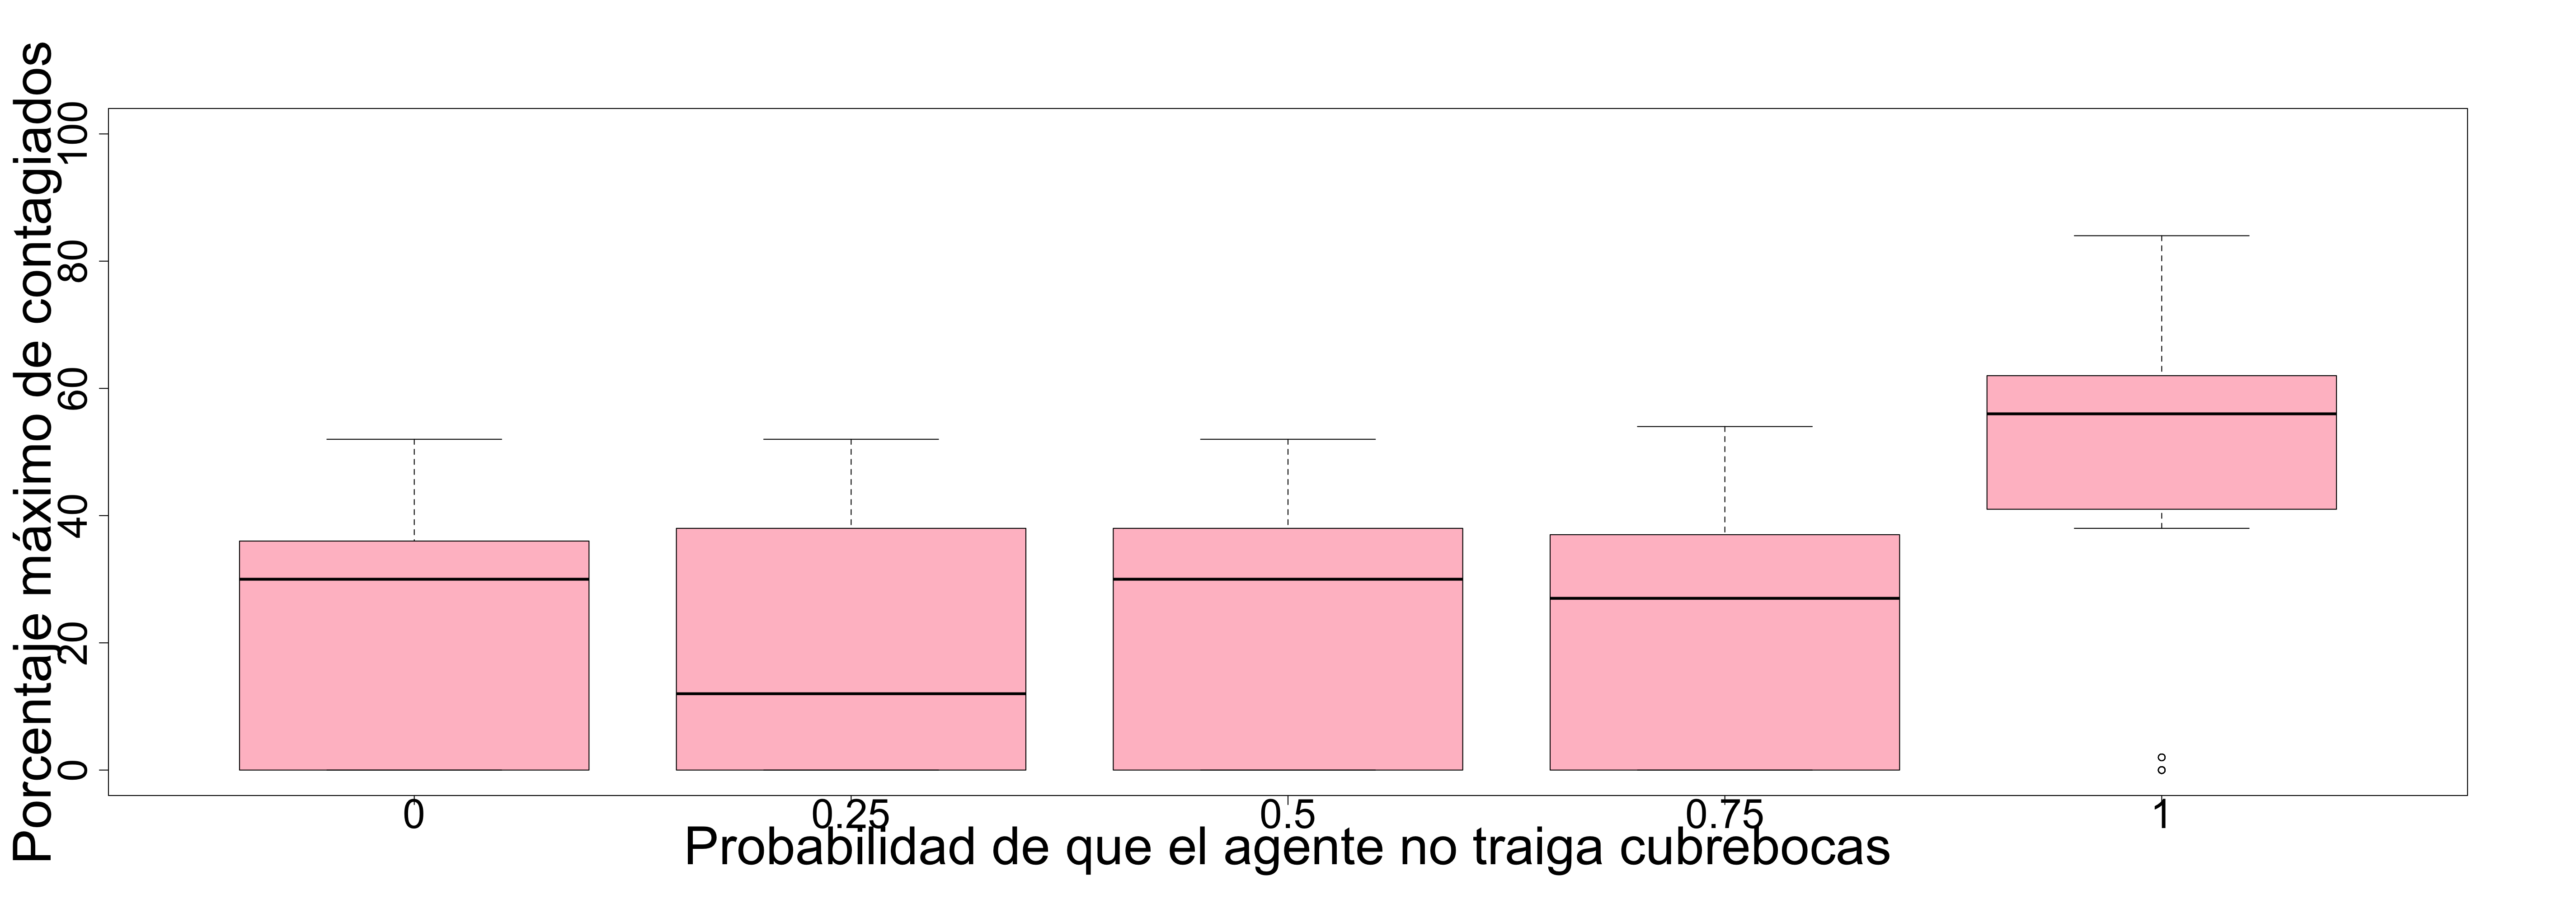
\includegraphics[width=\linewidth]{boxplot3.png}
\caption{Gráficos de caja variando la probabilidad de que un agente no use cubrebocas en el experimento 2.}
\end{figure}
\section{Conclusiones}
\begin{table}
\centering
\label{pvalue}
\caption{Valores $p$ obtenidos al realizar una prueba de T de Student.}
\begin{tabular}{|c|r|}
\hline 
Conjuntos & Valor $p$ \\ 
\hline 
1 - 2 & 0.2065 \\ 
\hline 
2-3 & 0.0468 \\ 
\hline 
3-4 & 0.3030 \\ 
\hline 
4-5 & 0.6909 \\ 
\hline 
\end{tabular} 
\end{table}
En el presente se trabajó con una simulación utilizando un sistema multiagente para verificar si existe un cambio significativo en el porcentaje de agentes contagiados si estos hacen uso de cubrebocas. La figura \ref{conmasc2} muestra que sí existen mejoras en el uso de los cubrebocas, para comprobarlo se realizan pruebas T de Student para revisar si hay diferencia significativa entre las medias de los conjuntos de datos obtenidos. El cuadro \ref{pvalue} muestra los valores $p$ obtenidos de dichas pruebas. Se concluye que cuando la probabilidad de que no traigan cubrebocas es muy grande, se tiene una diferencia significativa en el porcentaje máximo de contagiados.

A este modelo le hace falta tomar en cuenta muchos factores, como lo son el tipo de enfermad (epidemia) con la que se trata, algunas características de los agentes como el hecho de si poseen alguna enfermedad (cáncer, asma, diabetes, etcétera) que haga que el contagio sea más grave para él. Se podría mejorar la eficiencia del algoritmo utilizando, quizá, paralelismo. 
\subsection{Trabajo futuro}
Como trabajo a futuro se puede considerar la implementación de los aspectos mencionados anteriormente, así como también ampliar el entorno de los agentes a no una sola \textit{región}, es decir, que existan los \textit{viajes} entre diferentes zonas donde cada una tenga una diferente probabilidad de contagio. Referente al tema del uso del cubrebocas, también se podría considerar si el agente hace uso correcto de este o qué tipo utiliza. 
Tratar de implementar diferentes medidas sanitarias, como lo podría ser una cuarentena y así trabajar con otro tipo de modelo.
\bibliographystyle{elsarticle-num-names}
\bibliography{Referencias}




\end{document}
